Amelia is studying modeling. She is interested in models with moving parts.

As her first task, she made a rectangular box of size $2 \times n$, which contains two parallel rails and a rectangular bar on each of them. The short bar has size $1 \times a$, and the long one has size $1 \times b$. The long bar has a stopper at each end, and the short one is always between these two stoppers.

\begin{center}
\begin{tabular}{ccc}

\includegraphics{bars-1.ps} & 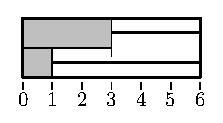
\includegraphics{bars-2.ps} & 
\includegraphics{bars-3.ps} \\
Example position & Initial position & Target position \\
\end{tabular}
\end{center}

The bars can be moved along the rails, one bar at a time, as long as the short bar is between the stoppers. So, on each \textit{move} Amelia selects one of the bars and moves it, while the other one stays in place.

Initially, both bars are aligned to one side of the box, and Amelia wants them to be aligned to the other side in as few moves as possible. What is the minimal number of moves she should do to achieve her goal?